\section{The IP Camera}
The type of robot we're dealing with is analagous to a human; It needs arms, legs, and eyes in order to work. However, during competition, eyes are perhaps more crucial than arms and legs, as they are all we have to determine decisions, collisions, and position. In the real world, these "eyes" come in the form of sensors and our own eyes, with the former being much more difficult to achieve accurately.

In most of our past competitions, sensors were a big issue. Mainly, it was down to inaccurate encoders or extremely laggy cameras, both which were massive challenges during competition. This experiment will deal with fixing the latter by looking at various options, with \autoref{section:accu_encoders} covering the former.

\subsection{The FPV Option}
Our goal: have low-latency, preferably cheap cameras that output a usable video quality wirelessly over a small distance. For all intents and purposes, this can be considered any FPV system, also known as a radio-controlled camera\cite{FPVWikipedia}.

\begin{figure}[h]
    \centering
    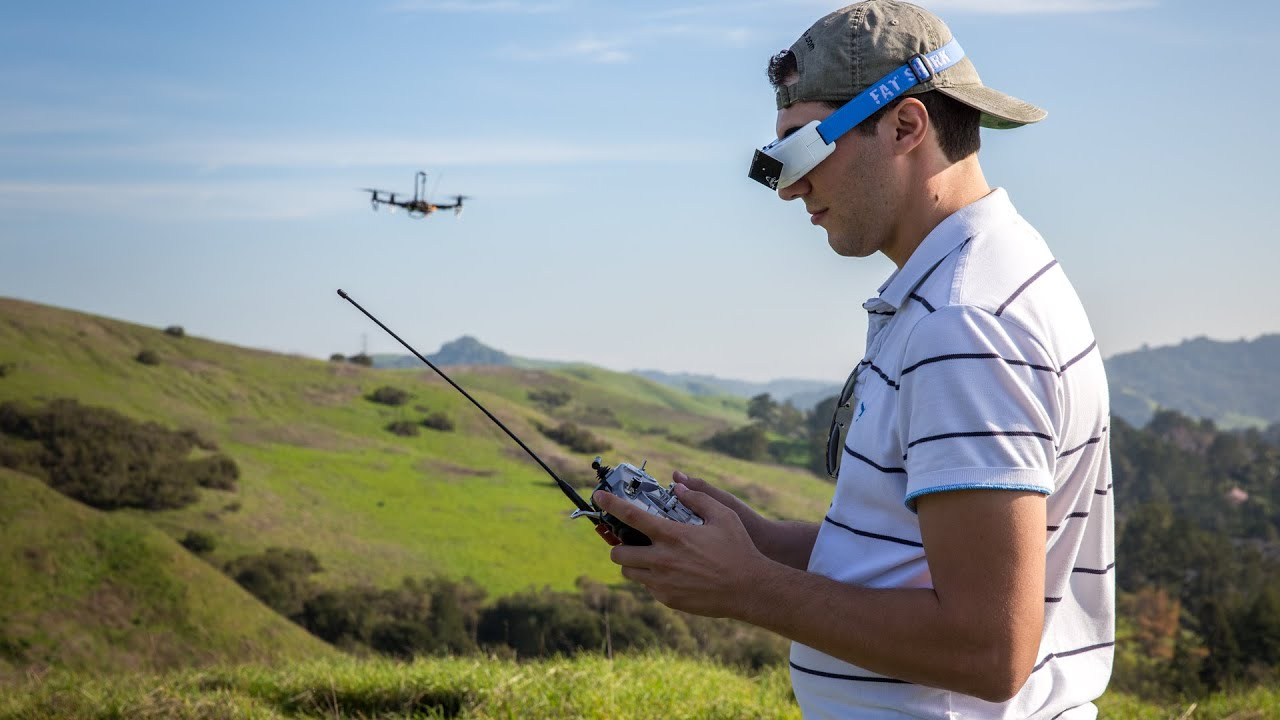
\includegraphics[width=\textwidth,height=6cm,keepaspectratio=true]{analogFPV}
    \caption{
        Screenshot of a drone FPV system from Adam Savage’s Tested \cite{analogFPV}.
    }
\end{figure}

One of the first things that may come to mind when dealing with this issue is looking at preexisting FPV systems. Specifically, analog FPV systems that transmit video over radio waves that can travel large distances. Most FPV systems on the market are targeted toward bringing real-time video at HD quality wirelessly, so why not use these?

The main issue at avoiding quality FPV systems is cost. Simply put, FPV systems are largely meant for long-distance, airborne transmission. In fact, one of the most popular FPV systems to date, DJI \cite{DJI}, aims to bring real-time HD video with a latency less than 28ms over distances upwards to 4 kilometers. Its cost however, as of February 2021, comes to a bit more than 400\$ just including the googles, the camera, and antennas; A bit too much for our purposes.

So why not use nanny cameras? After all, some nanny cameras \cite{nannyCam} can transmit HD video wirelessly while being at a reasonable price.

While nanny cameras might be the perfect size for our scenario, they are not advertised at being low-latency. Instead, nanny cameras are mostly used for security purposes, meaning that they are mainly designed to record video, not stream it at low-latencies. Due to this, they are not considered a reliable camera for our purposes, and so we will be avoiding them.


\subsection{The Mobile Option}

Maybe we can find a way to achieve cheap, low-latency streaming in mobile phones; a technology that is already prominent in America. In particular, there a wide range of Android apps that can be used to stream video from the camera to another device. For this section, we will only consider the following:

\begin{itemize}
\item Skype
\item Jami
\item IP Camera

\end{itemize}
